\chapter{Implementasi dan Pengujian}
\label{chap:implementasi&pengujian}

Pada bab ini akan dijelaskan mengenai implementasi perangkat lunak, serta pengujian perangkat lunak. Implementasi perangkat lunak berisi penjelasan lingkungan pengembangan perangkat lunak dan hasil implementasi. Sedangkan pengujian perangkat lunak berisi hasil pengujian fungsional dan eksperimental terhadap perangkat lunak yang telah dibangun.

\section{Implementasi}

\subsection{Lingkungan Implementasi}
\label{lingkungan_implementasi}
Implementasi perangkat lunak ini dilakukan di komputer penulis dengan spesifikasi berikut:
\begin{enumerate}
    \item \textit{Processor}: Intel Core i5-10300H
    \item \textit{Random Access Memory(RAM)}: 16 GB DDR4
    \item Sistem Operasi: Windows 10
    \item Versi Java: 1.8.0\_291
    \item Versi JavaFX: 8.0.291
    \item Versi Netbeans: 12.1
    \item Versi Scenebuilder: 11.0.0
\end{enumerate}

\subsection{Hasil Implementasi}
Hasil implementasi berupa sebuah \textit{file} yang berekstensi \textbf{jar}. Agar dapat digunakan sebagai \textit{screensaver}, \textit{file} tersebut perlu diubah ekstensinya menjadi \textbf{scr}. Untuk mengubah ekstensi menjadi \textbf{scr}, perlu dilakukan perubahan menjadi ekstensi \textbf{exe} terlebih dahulu. Perubahan ekstensi menjadi \textbf{exe} tersebut dilakukan dengan bantuan aplikasi bernama Launch4j\footnote{\url{http://launch4j.sourceforge.net}}. Setelah didapatkan \textit{file} berekstensi \textbf{exe}, maka untuk mengubahnya menjadi berekstensi \textbf{scr} cukup dengan melakukan rename pada file tersebut menjadi berekstensi \textbf{scr}. File berekstensi \textbf{scr} tersebut dapat disimpan pada direktori ``System32'' didalam folder ``Windows'' agar dapat terdeteksi sebagai \textit{screensaver} oleh Windows. Setelah mengatur aplikasi menjadi \textit{screensaver}, aplikasi tersebut akan dijalankan secara otomatis setelah komputer tidak digunakan selama beberapa saat. Gambar \ref{fig:5_hasil} dan \ref{fig:5_hasil2} merupakan tampilan dari aplikasi \textit{screensaver}. Dikarenakan pada Portal Akademik Mahasiswa tidak terdapat foto mahasiswa, maka foto digantikan dengan \textit{base64 image} yang dimasukkan secara \textit{hardcode}. \textit{Layout} dari aplikasi disimpan dalam \textit{file} bertipe FXML (lampiran \ref{lamp:E}). \textit{File} FXML tersebut tidak dibuat secara manual, melainkan dengan menggunakan aplikasi Scene Builder\footnote{\url{https://gluonhq.com/products/scene-builder/}}. 

\begin{figure}[H]
	\centering
	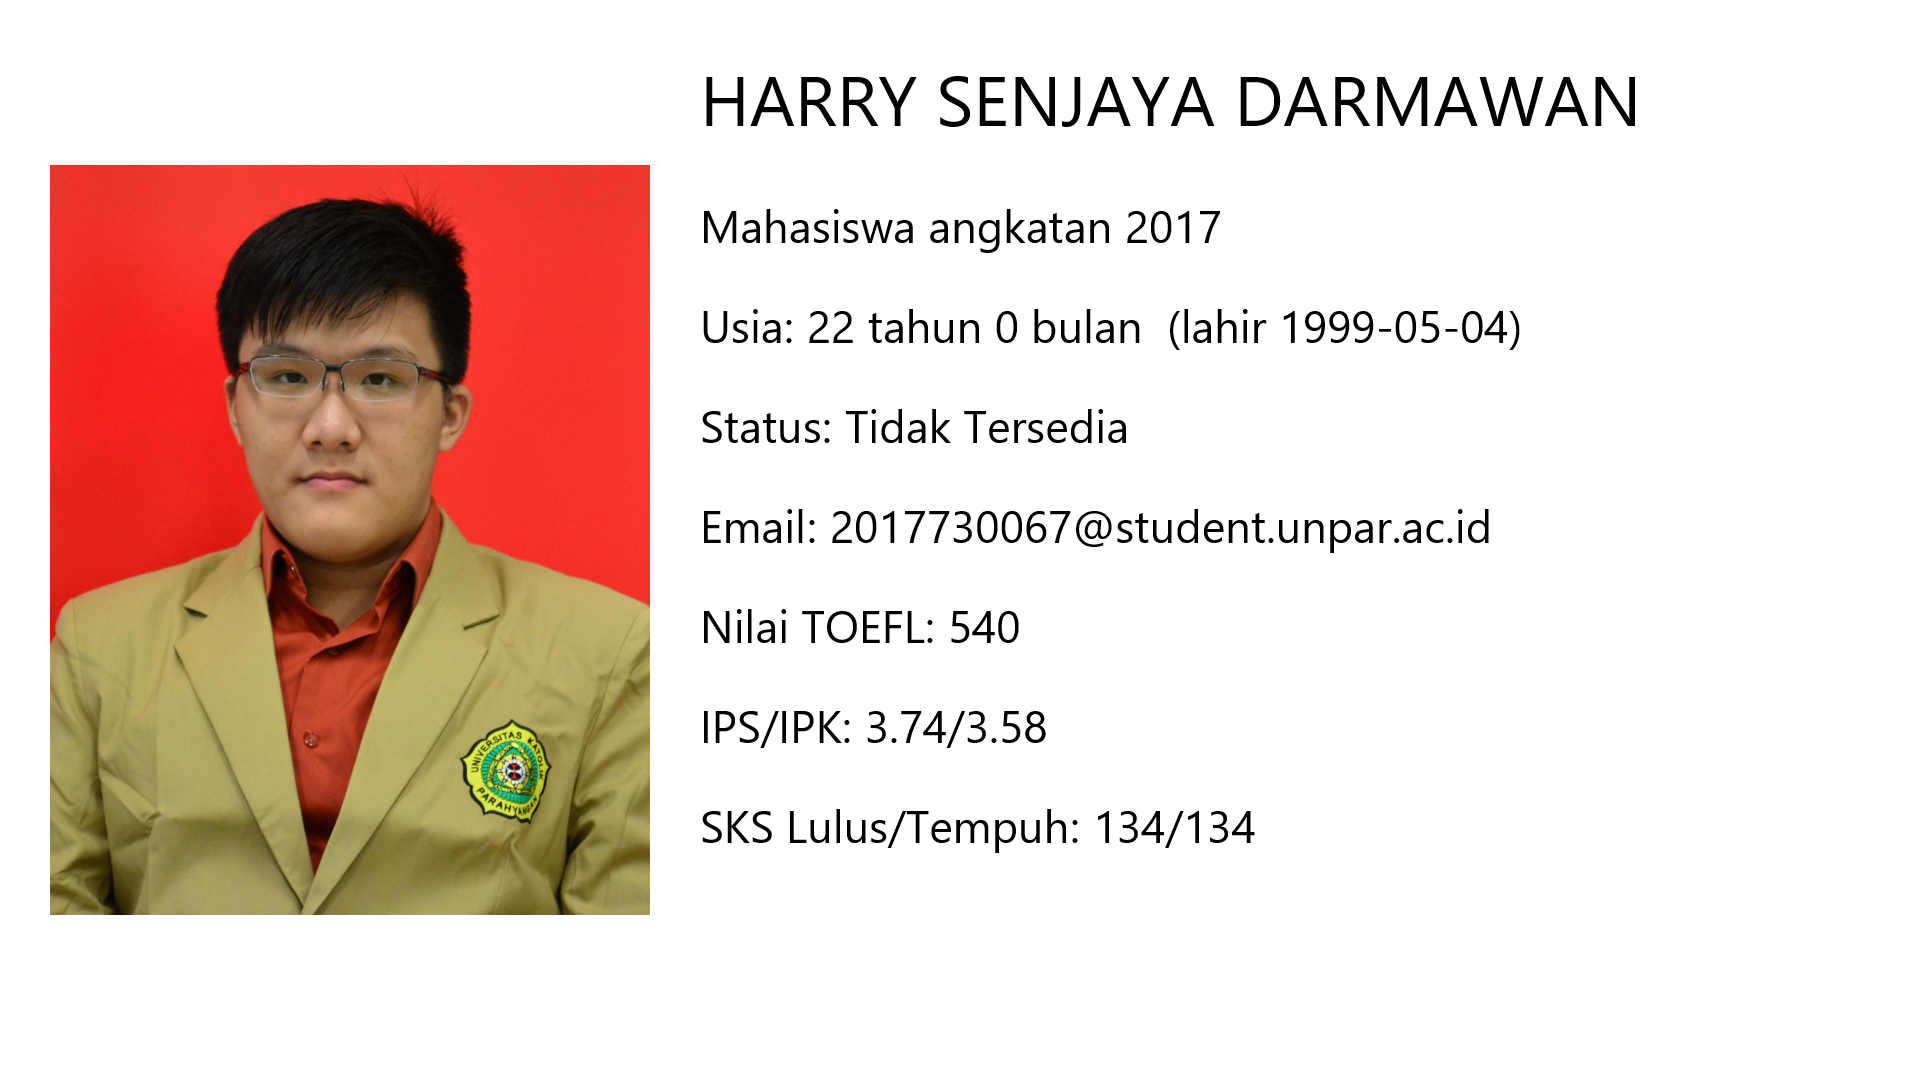
\includegraphics[scale=0.3]{Gambar/hasil.png}
	\caption{Tampilan \textit{Screensaver} Mahasiswa Pertama}
	\label{fig:5_hasil}
\end{figure}

\begin{figure}[H]
	\centering
	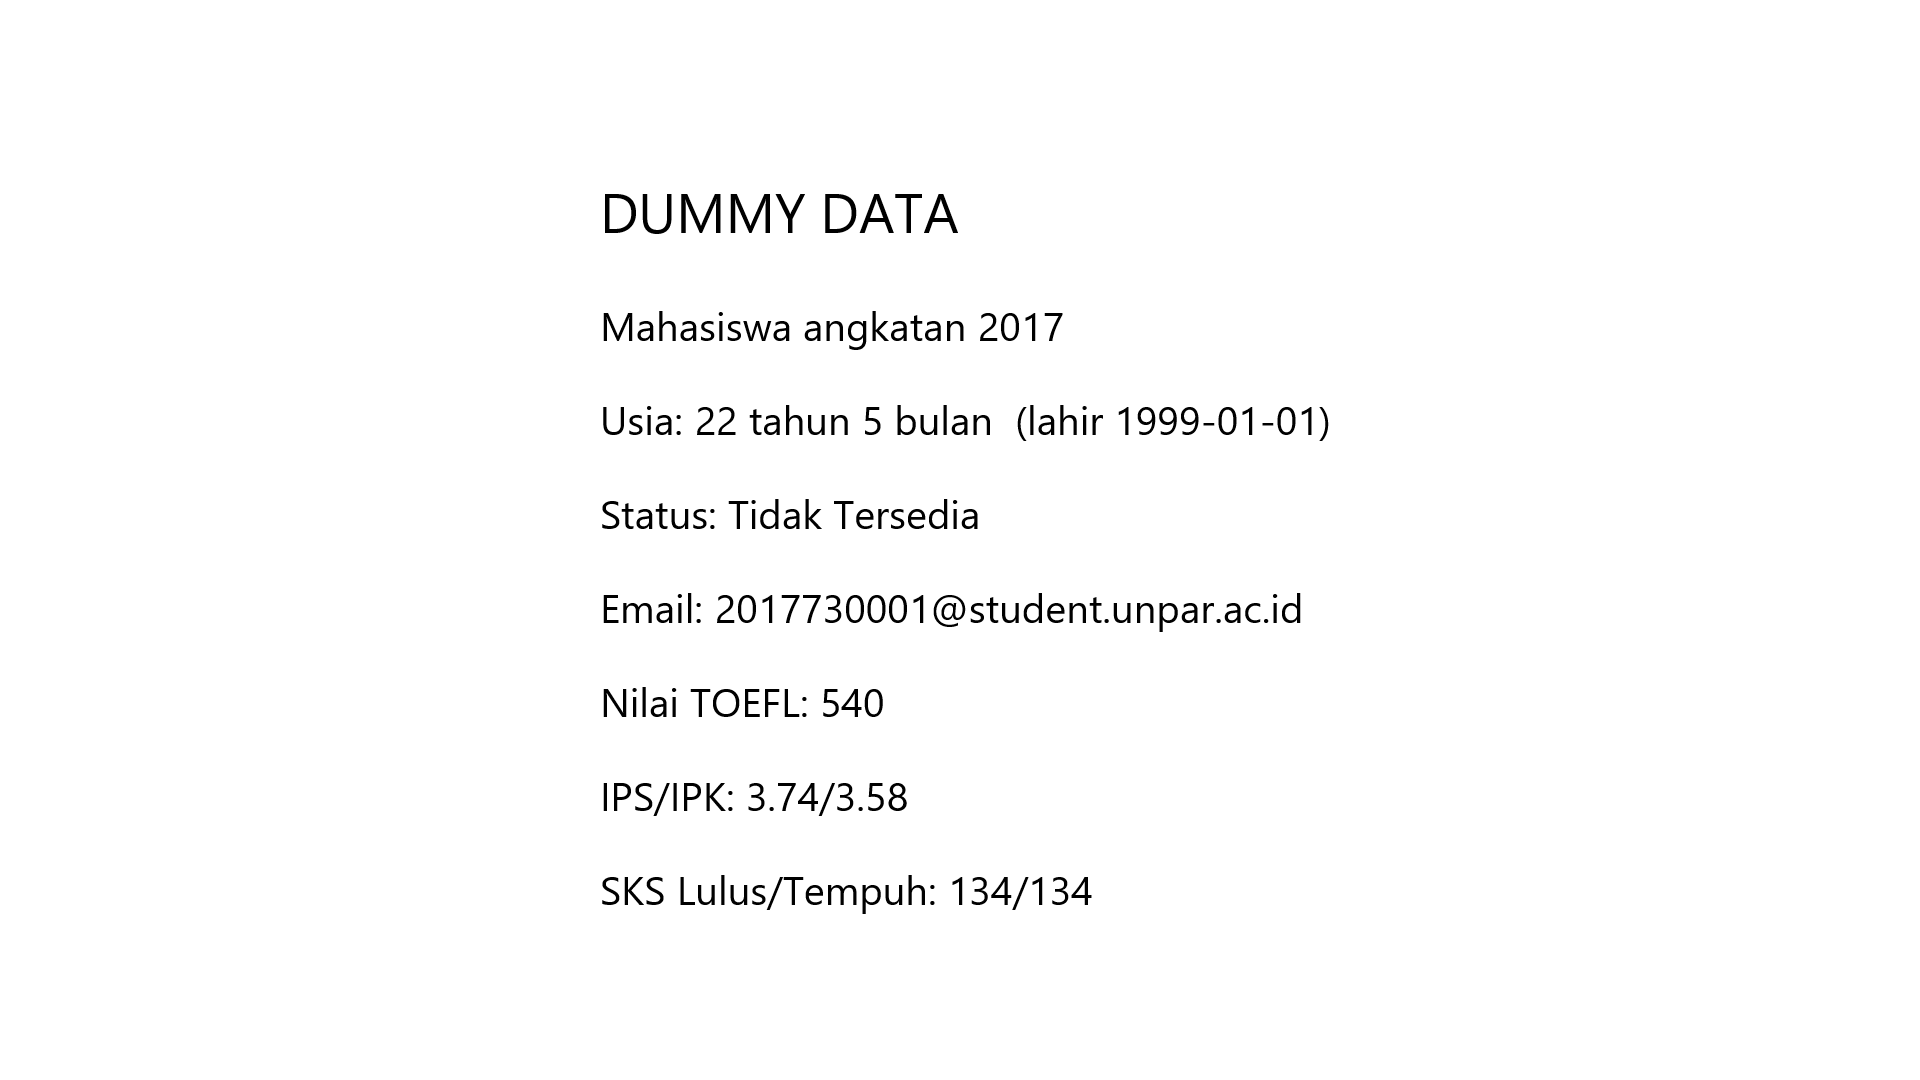
\includegraphics[scale=0.3]{Gambar/hasil2.png}
	\caption{Tampilan \textit{Screensaver} Mahasiswa Kedua}
	\label{fig:5_hasil2}
\end{figure}


\section{Pengujian}

\subsection{Pengujian Fungsional}
Pengujian fungsional dilakukan untuk mengetahui kesesuaian reaksi perangkat lunak dengan reaksi yang diharapkan berdasarkan aksi pengguna terhadap perangkat lunak. Tabel \ref{table:hasilFungsional} merupakan hasil pengujian perangkat lunak yang dilakukan di komputer penulis dengan spesifikasi berikut:
\begin{enumerate}
    \item \textit{Processor}: Intel Core i5-10300H
    \item \textit{Random Access Memory(RAM)}: 16 GB DDR4
    \item Sistem Operasi: Windows 10
    \item Resolusi Layar: 1920 x 1080
    \item Versi Java: 1.8.0\_291
\end{enumerate}

\begin{table}[H]
	\centering
	\caption{Tabel Pengujian Fungsional}
	\begin{tabular}{|p{0.5cm}| p{5.5cm}| p{5.5cm}| p{3cm}|} \hline
	No.	&	Aksi Pengguna	&	Reaksi yang diharapkan	&	Reaksi Perangkat Lunak \\ \hline
	1 	& Dosen tidak menggunakan komputer selama beberapa saat, dengan kondisi  koneksi internet berfungsi dengan normal.  	&	\textit{Screensaver} berjalan dengan menampilkan biodata dan data akademik mahasiswa wali secara umum. &	sesuai	\\ \hline
	2 	& Dosen tidak menggunakan komputer selama beberapa saat, dengan kondisi koneksi internet tidak berfungsi dengan normal. 	&	\textit{Screensaver} berjalan dengan menampilkan peringatan bahwa koneksi internet tidak berfungsi dengan normal. &	sesuai	\\ \hline 	
	3 	& Mahasiswa tidak menggunakan komputer selama beberapa saat, dengan kondisi  koneksi internet berfungsi dengan normal. 	&	\textit{Screensaver} berjalan dengan menampilkan biodata dan data akademik mahasiswa secara umum beserta dengan data dummy. &	sesuai	\\ \hline 
	4 	& Mahasiswa tidak menggunakan komputer selama beberapa saat, dengan kondisi koneksi internet tidak berfungsi dengan normal. 	&	\textit{Screensaver} berjalan dengan menampilkan peringatan bahwa koneksi internet tidak berfungsi dengan normal. &	sesuai	\\ \hline 
	\end{tabular}
	\label{table:hasilFungsional}
\end{table}


\subsection{Pengujian Eksperimental}
\textit{Subbab ini ditulis oleh dosen pembimbing.}

Pengujian eksperimental dilakukan oleh dosen pembimbing, karena mahasiswa tidak memiliki akses ke SIAKAD apalagi ke data mahasiswa di luar penulis sendiri. Pengujian eksperimental dilakukan dengan melakukan \textit{git branching} dari hasil (hampir) final dari penulis di commit \texttt{d60be65}. Pengujian eksperimental dilakukan pada komputer dosen dengan spesifikasi seperti berikut\footnote{Idealnya pengujian dilakukan di komputer UNPAR dengan sistem operasi Microsoft Windows sehingga bisa benar-benar digunakan sebagai \textit{screensaver}. Namun, karena keadaan pandemi sehingga dosen tidak bisa mengunjungi UNPAR dan hanya bisa melakukan pengujian di rumah dengan komputer macOS}:

\begin{enumerate}
	\item Komputer: iMac (21.5-inch, Late 2013)
    \item Sistem Operasi: macOS Catalina 10.15.7
    \item \textit{Processor}: 2,7 GHz Quad-Core Intel Core i5
    \item \textit{Memory}: 8 GB 1600 MHz DDR3
    \item \textit{Graphics}: Intel Iris Pro 1536 MB
    \item Resolusi Layar: 1920 x 1080
    \item Versi Java: 1.8.0\_282
\end{enumerate}

Ada beberapa penyesuaian yang dilakukan oleh dosen pembimbing supaya \textit{screensaver} bisa dijalankan dengan cukup baik pada lingkungan dosen. Karena keterbatasan waktu, penyesuaian ini dilakukan tanpa berkoordinasi secara intensif dengan mahasiswa. Penyesuaian-penyesuaian tersebut antara lain:

\begin{enumerate}
	\item \textbf{Data diambil dari SIAKAD bukan dari Portal Akademik Mahasiswa.} Daftar mahasiswa yang diambil diacak urutannya sehingga saat ditampilkan tidak selalu dimulai dari angkatan tertua.
    \item \textbf{Upgrade versi SIAModels dari 4.0.0 menjadi 5.0.1.} Pada versi terbaru SIAModels, ada beberapa perbaikan, di mana salah satunya adalah \textit{bug} saat menentukan angkatan mahasiswa berdasarkan NPM nya. Perbaikan lainnya adalah pada perhitungan IPK dan IPS. SIAModels merupakan pustaka eksternal dan bukan merupakan bagian inti dari \textit{screensaver} yang dibuat.
    \item \textbf{Load data di \textit{thread} terpisah.} Pada program yang dibuat oleh mahasiswa, program hanya mengunduh satu data dari Portal Akademik Mahasiswa, yaitu data yang bersangkutan sendiri. Pada SIAKAD, diunduh banyak data dan ternyata menimbulkan masalah saat mengunduh data mahasiswa untuk ditampilkan pada slide berikutnya. Masalah muncul karena saat load data mahasiswa berikutnya, program menjadi tidak responsif. Oleh karena itu, saat menampilkan sebuah slide, program diubah supaya mengunduh data mahasiswa untuk slide berikutnya di latar belakang. Saat slide berikutnya ditampilkan, sudah tidak perlu melakukan pengunduhan kembali karena datanya sudah siap.
    \item \textbf{Saat mengulang ke mahasiswa pertama, tidak dilakukan load data kembali.}
    \item \textbf{Jika data mahasiswa belum siap ditampilkan, tidak maju ke slide berikutnya.}
    \item \textbf{\textit{Bugfix} untuk pembacaan bulan Februari.} Pada SIAKAD, ternyata bulan kedua dituliskan sebagai ``Pebruari'' dengan huruf ``P'', karena itu perlu penyesuaian sehingga mahasiswa dengan bulan lahir Februari dapat dibaca dengan baik.
\end{enumerate}

Perubahan lengkap kode dibandingkan dengan kode milik mahasiswa dapat dilihat pada lampiran \ref{diff_dosen_mahasiswa}.
Setelah perbaikan-perbaikan tersebut dilakukan, program dapat dijalankan dengan baik, dan untuk menampilkan 30 mahasiswa ``wali'' dari dosen pembimbing, dibutuhkan waktu sekitar 8 menit, di mana setelahnya mengulang kembali dari mahasiswa pertama. Beberapa hasil tangkapan layar dapat dilihat pada gambar \ref{fig:5_ss1}, \ref{fig:5_ss2}, \ref{fig:5_ss3}, \ref{fig:5_ss4}, dan \ref{fig:5_ss5}. Dosen sudah meminta izin kepada kelima mahasiswa tersebut untuk datanya dapat ditampilkan pada laporan ini, melalui e-mail.

\begin{figure}[H]
	\centering
	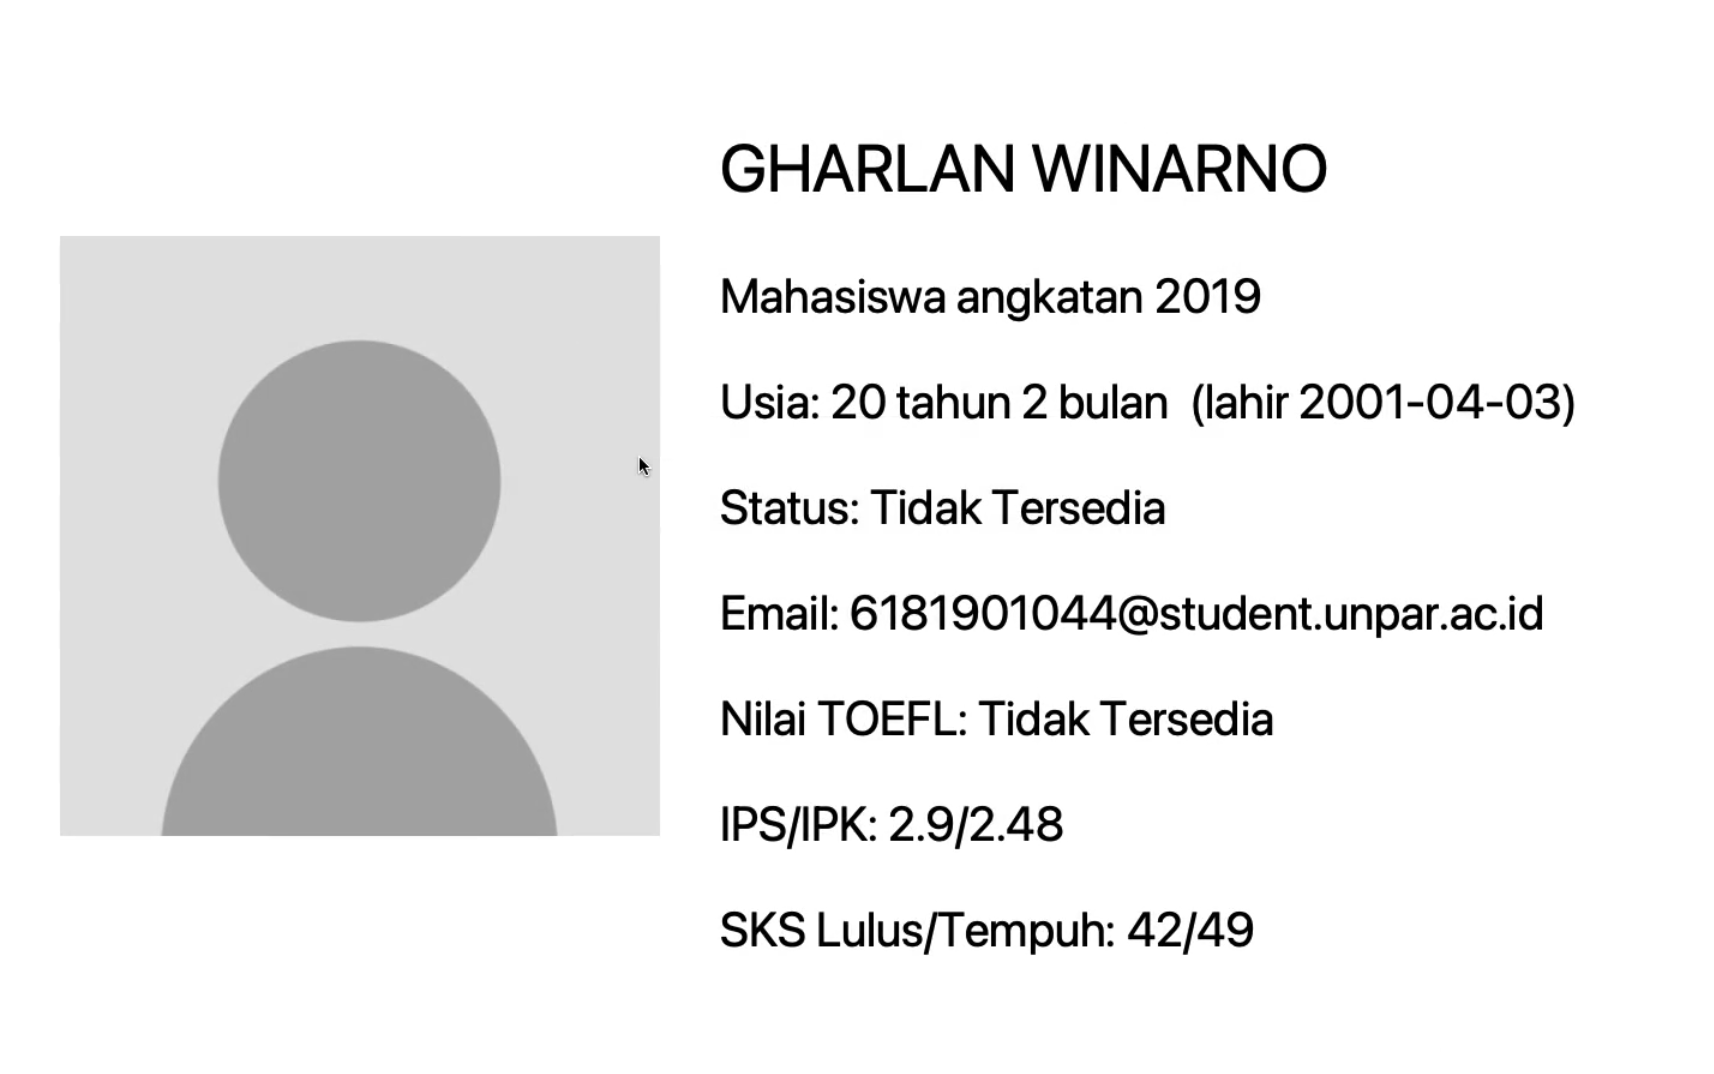
\includegraphics[scale=0.25]{Gambar/ss1.png}
	\caption{Tampilan \textit{Screensaver} Mahasiswa Pertama}
	\label{fig:5_ss1}
\end{figure}

\begin{figure}[H]
	\centering
	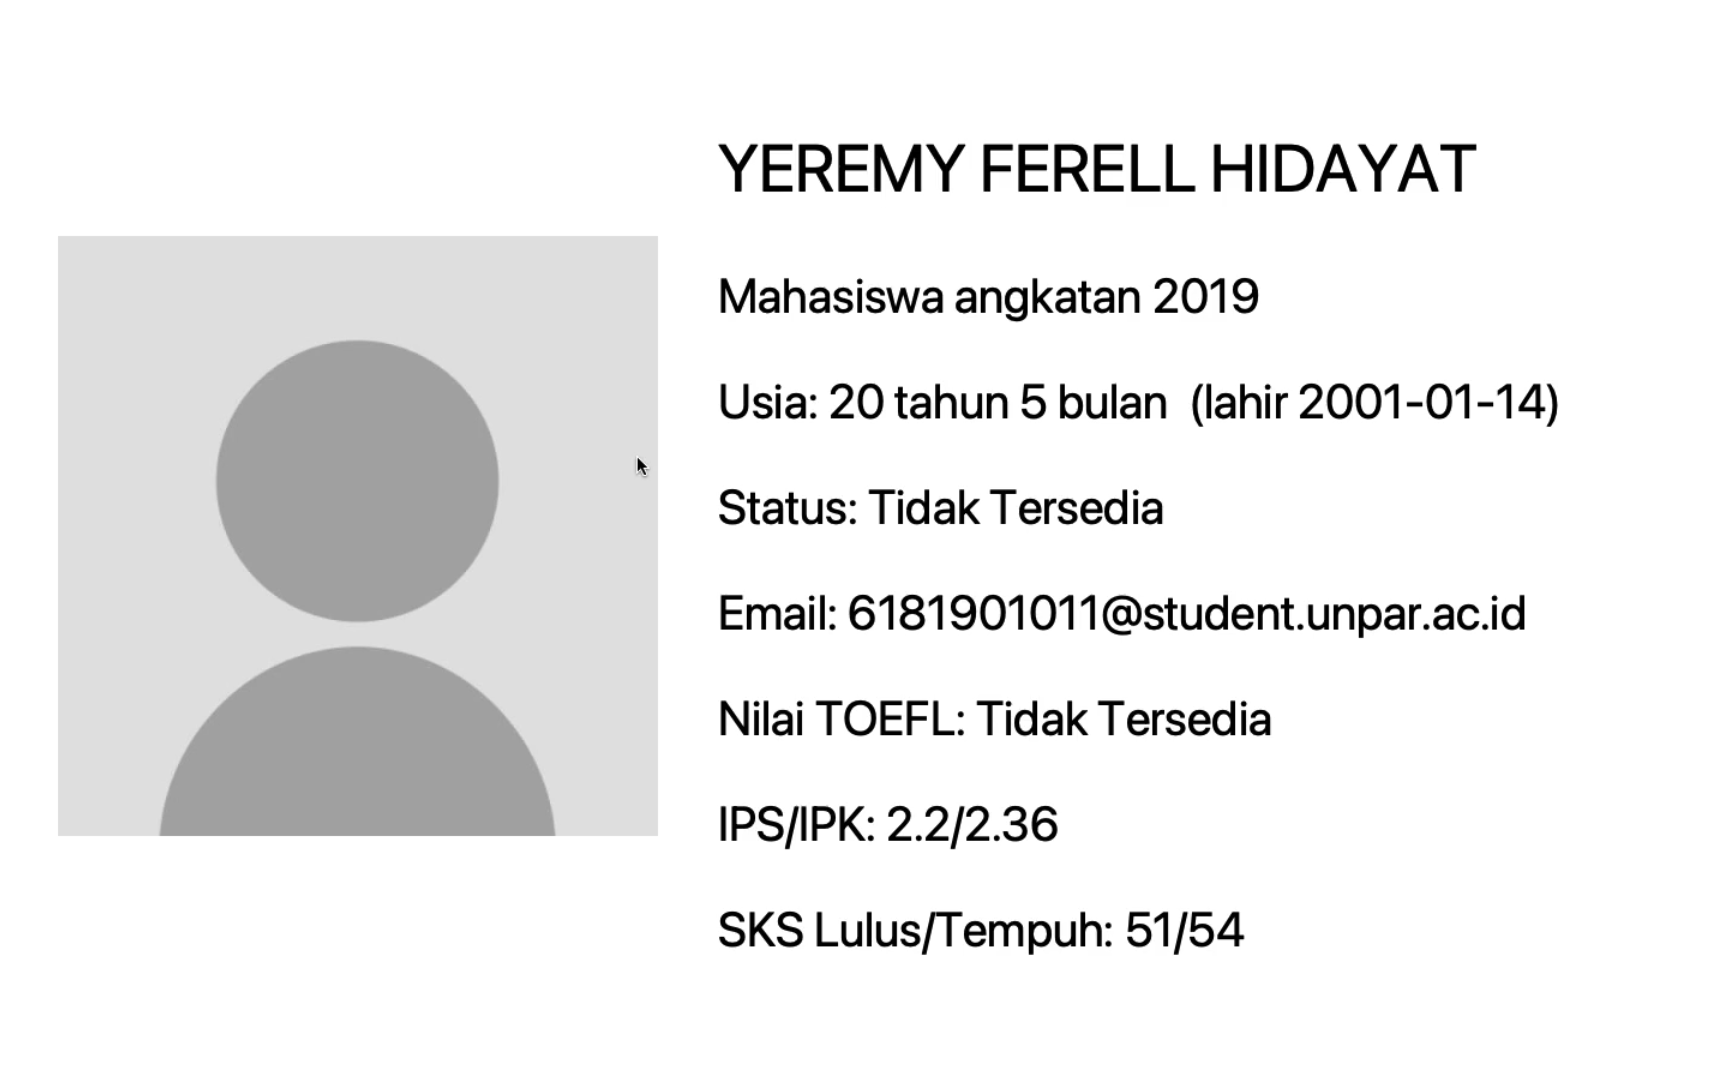
\includegraphics[scale=0.3]{Gambar/ss2.png}
	\caption{Tampilan \textit{Screensaver} Mahasiswa Kedua}
	\label{fig:5_ss2}
\end{figure}

\begin{figure}[H]
	\centering
	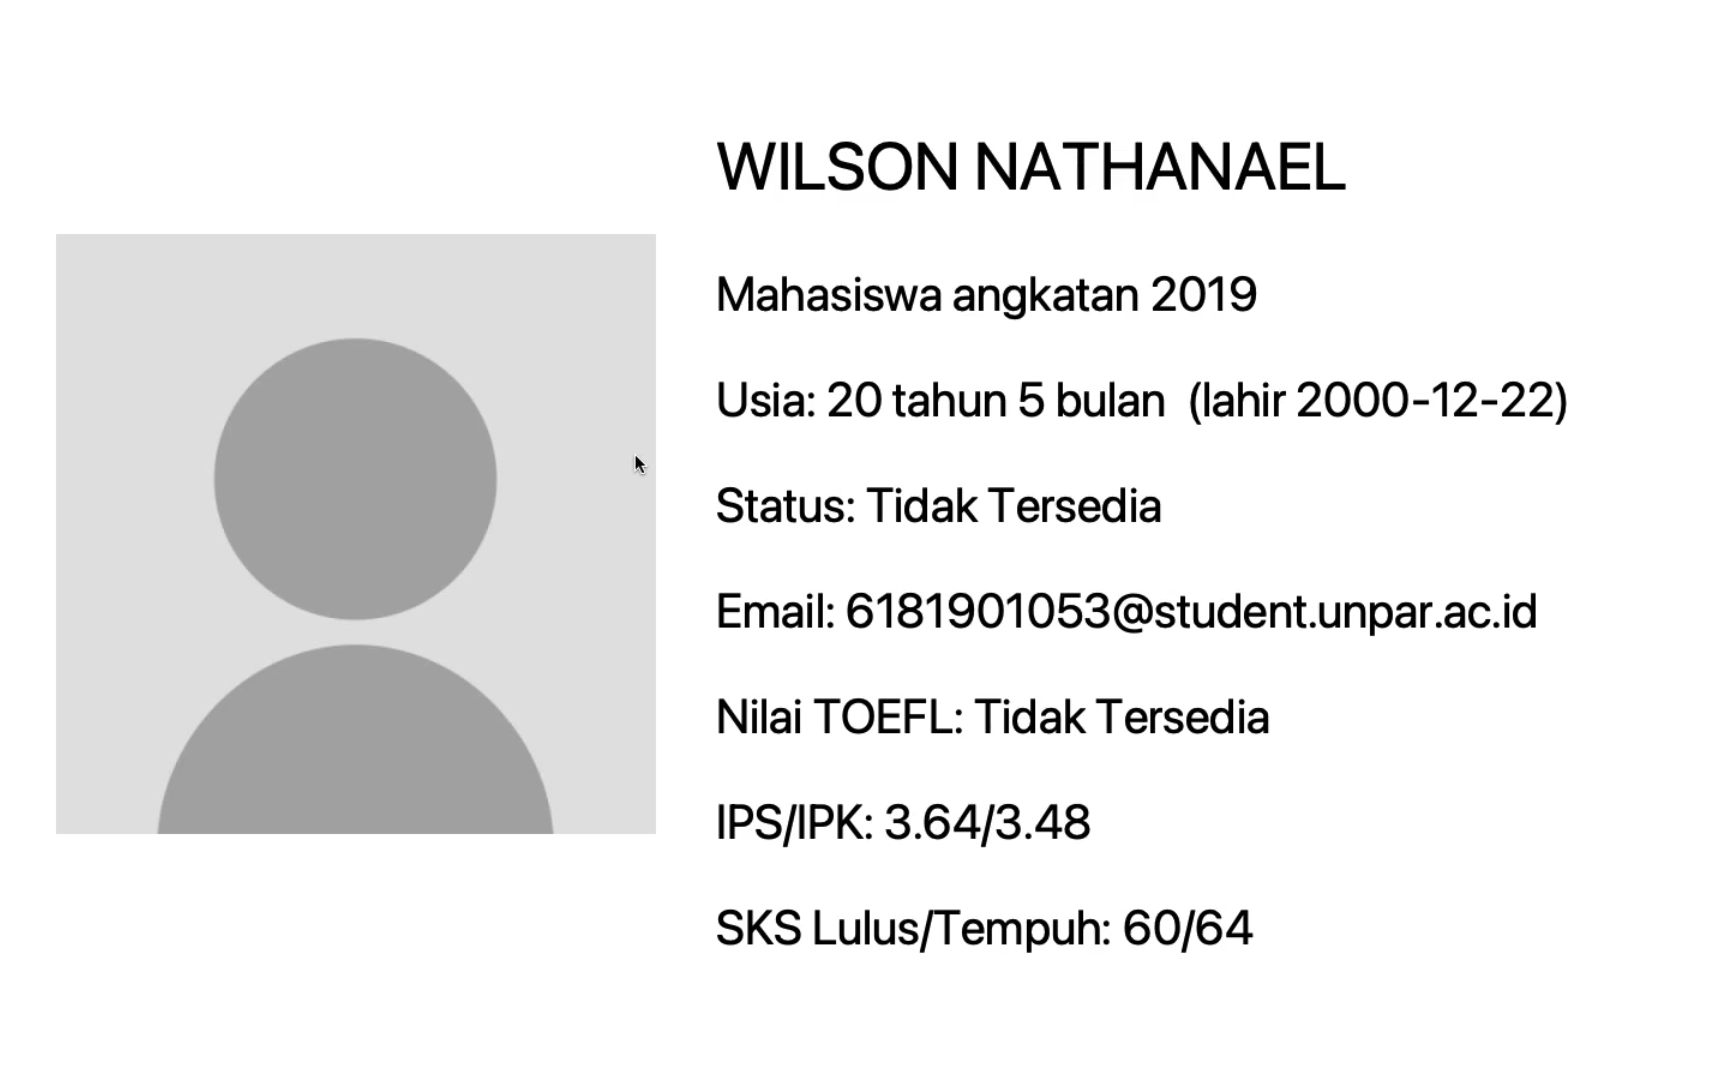
\includegraphics[scale=0.3]{Gambar/ss3.png}
	\caption{Tampilan \textit{Screensaver} Mahasiswa Ketiga}
	\label{fig:5_ss3}
\end{figure}

\begin{figure}[H]
	\centering
	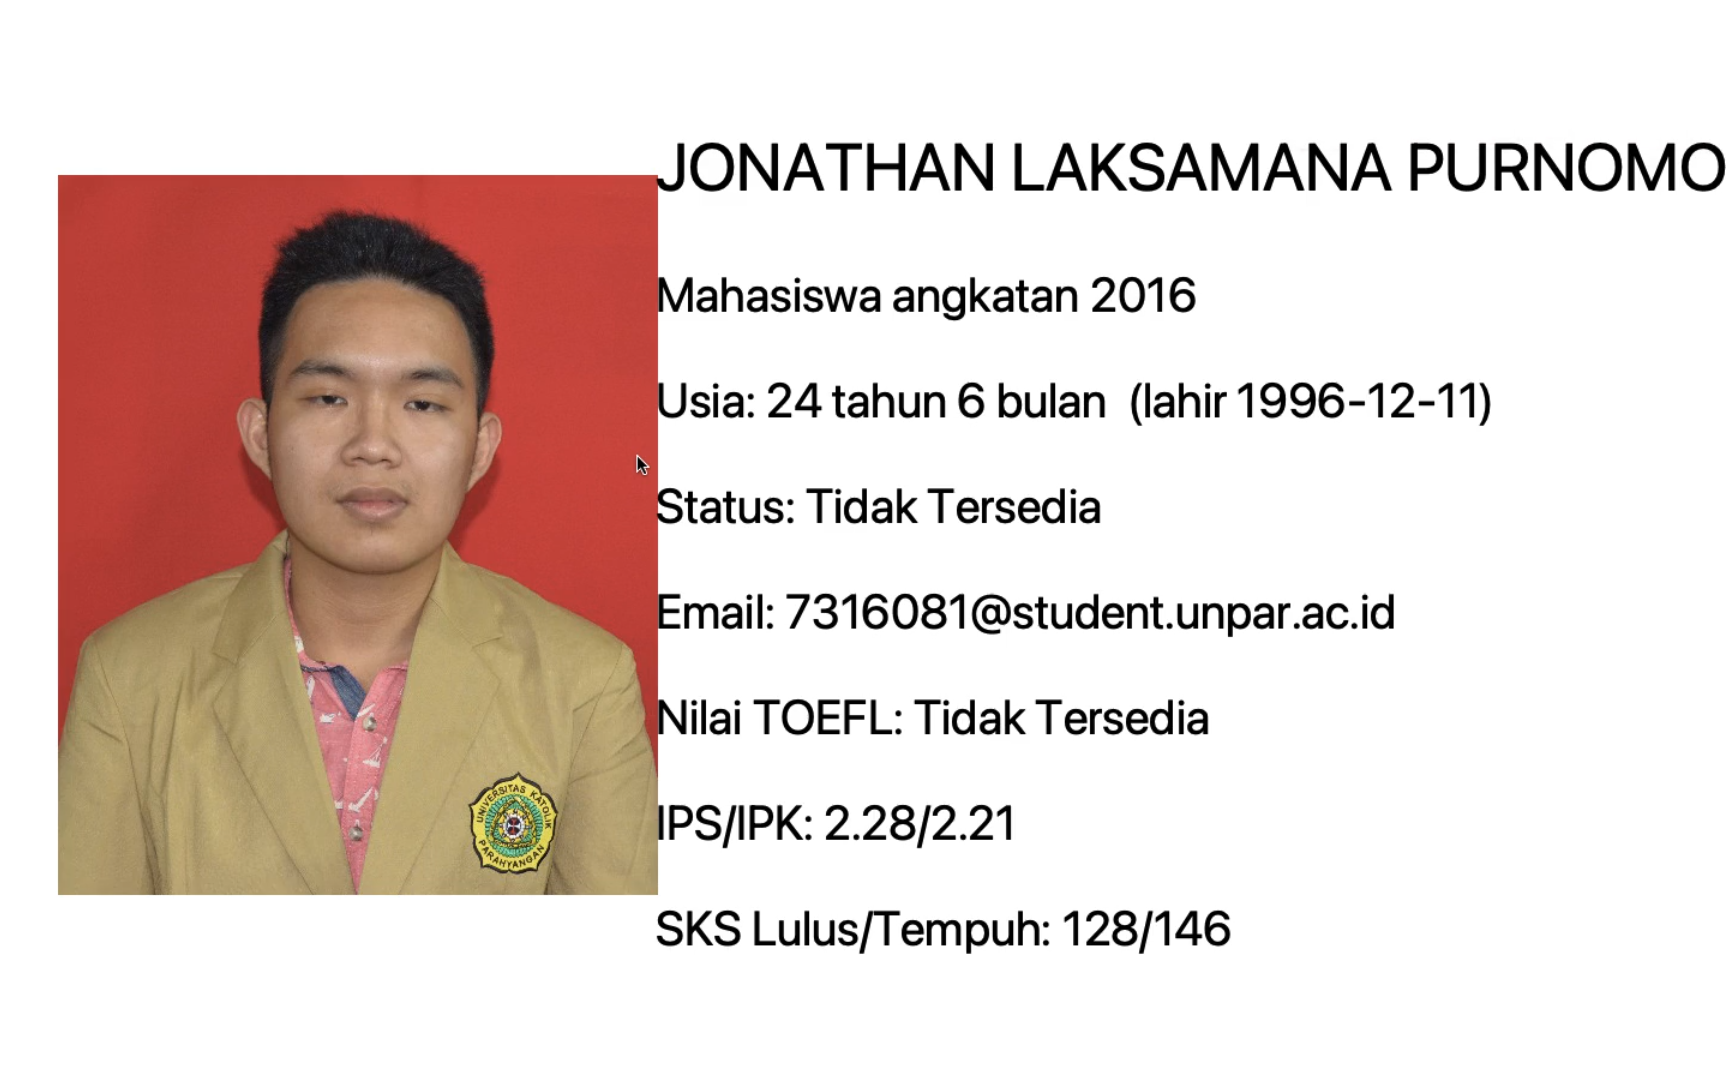
\includegraphics[scale=0.3]{Gambar/ss4.png}
	\caption{Tampilan \textit{Screensaver} Mahasiswa Keempat}
	\label{fig:5_ss4}
\end{figure}

\begin{figure}[H]
	\centering
	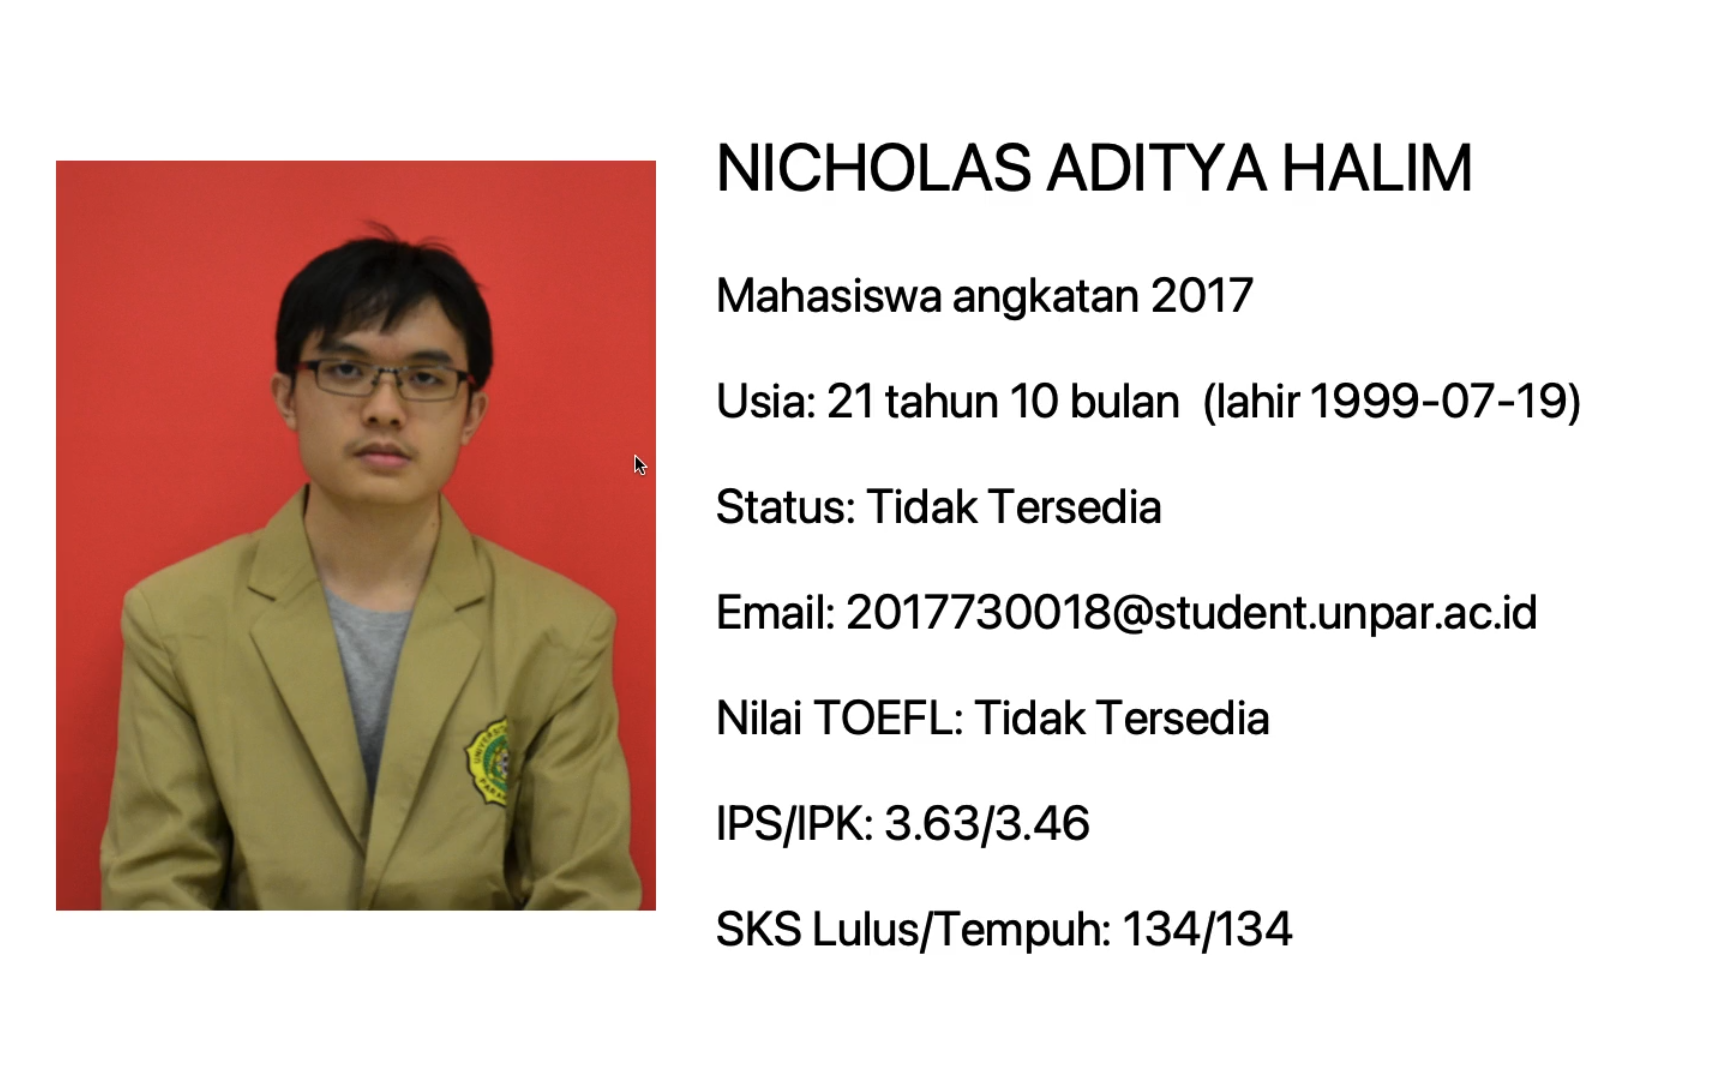
\includegraphics[scale=0.3]{Gambar/ss5.png}
	\caption{Tampilan \textit{Screensaver} Mahasiswa Kelima}
	\label{fig:5_ss5}
\end{figure}
